\chapter{Metode Penelitian}

\section{Arsitektur Aplikasi}

Aplikasi akan dibagi menjadi dua bagian yaitu \textbf{Frontend} (yang berhadapan di sisi pendengar atau pengakses) dan \textbf{Backend} (yang berurusan dengan penyiar). 

Pada bagian Frontend, pendengar akan berhadapan dengan server penyeimbang muat berbasis HAProxy yang akan mengarahkan permintaan pendengar ke server yang tersedia untuk melayani. Sementara pada bagian Backend, pengirim atau penyiar akan berhadapan dengan server penerima data aliran audio yang nantinya akan menyebarkan data audio ke seluruh server penyedia.

\begin{figure}
    \centering
    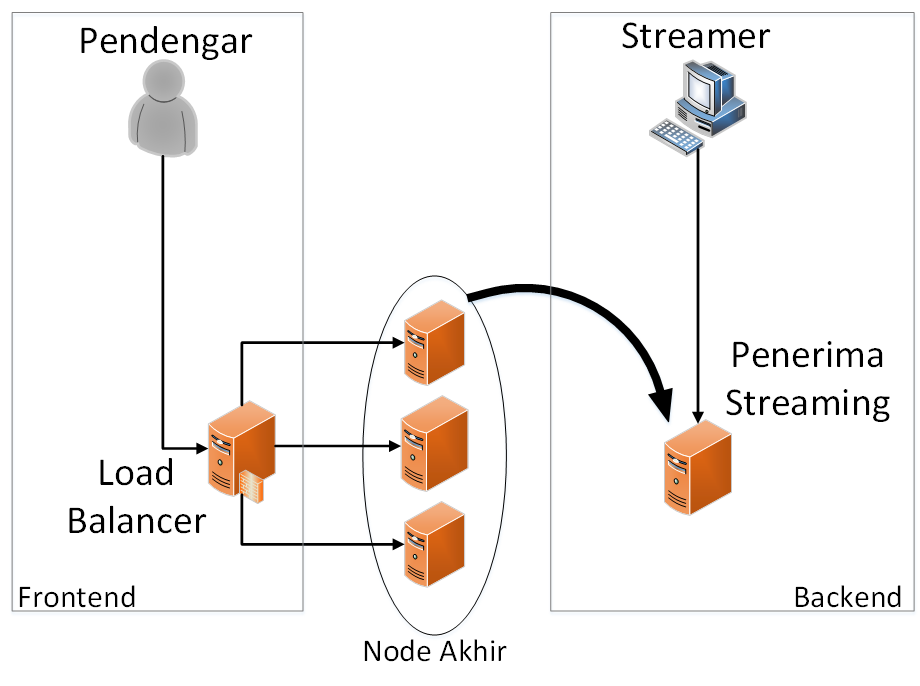
\includegraphics[width=0.5\linewidth]{arsitektur}
    \caption{Arsitektur Jaringan}
    \label{fig:arsitektur}
\end{figure}

Gambar \ref{fig:arsitektur}  menjelaskan bagaimana interaksi antara server (Frontend dan Backend), pendengar, dan pengirim. Dengan pembagian kerja ini nantinya pendengar hanya akan mengetahui aliran data audio mana saja yang aktif dan pengirim hanya akan mengirim aliran data audio.

\section{Fitur Aplikasi}
\subsection{Pengaliran Data Audio}

Perangkat lunak server IceCast pada awalnya hanya mendukung pengaliran data audio ke satu server saja untuk satu kali proses pengaliran. Fitur Pengaliran Data Audio dalam penelitian ini akan membuat pengaliran data audio tidak hanya tertuju ke satu server, melainkan ke banyak server sekaligus yang dikelola oleh sistem pembagi muat. Sistem akan dibuat setransparan mungkin sehingga pihak penyiar atau pengirim hanya tetap mengakses pengiriman data ke satu alamat server seperti sebelumnya.

Pada Gambar \ref{fig:kirim-server} diagram alir menjelaskan bagaimana pengirim mengirimkan paket audionya ke satu server saja. Pada saat data audio masuk ke server, server akan meneruskan data audio ke node akhir sehingga node akhir memiliki data audio yang sama dengan yang diterima server.

Gambar \ref{fig:kirim-server} menjelaskan apa yang terjadi di bagian backend aplikasi.

\begin{figure}
    \centering
    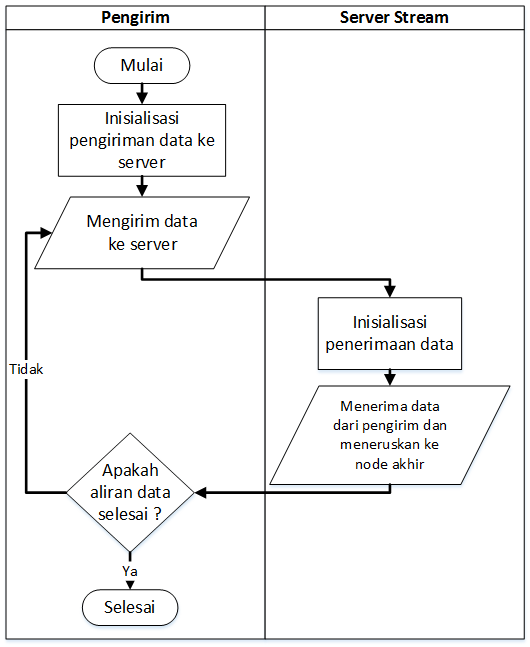
\includegraphics[width=0.7\linewidth]{kirim-server}
    \caption{Alur Kerja Pengirim dan Server}
    \label{fig:kirim-server}
\end{figure}


\subsection{Penyeimbang Muat}
Penyeimbang muat diakses ketika ada pendengar atau pengakses yang ingin mengakses siaran yang tersedia pada Server. Pada kenyataannya pendengar hanya akan mengakses satu alamat server yang akan memintakan layanan ke Node akhir. Server yang diakses oleh pendengar tidak memiliki layanan yang diminta oleh pendengar, server hanya bertindak sebagai penerus dan penyeimbang muat bagi permintaan yang banyak.

\begin{figure}
    \centering
    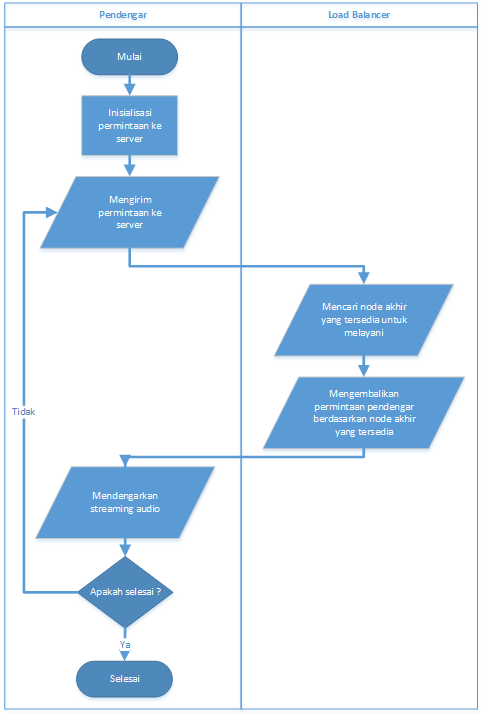
\includegraphics[width=0.7\linewidth]{dengar-server}
    \caption{Alur Kerja Pendengar dan Server}
    \label{fig:dengar-server}
\end{figure}

Sesuai dengan Gambar \ref{fig:dengar-server}, server yang diakses pengguna adalah server penyeimbang muat yang hanya sebagai jembatan dalam layanan aliran data audio. 

\section{Sarana Yang Digunakan}

Dalam penilitian ini, digunakan beberapa teknologi untuk mengaplikasikan rancangan yang sudah ada, diantaranya:

\begin{enumerate}
    \item Bahasa Pemrograman
    
    Menggunakan nodejs untuk konfigurasi antara pengirim dan server.
    
    \item Editor Teks
    
    Penilitian ini menggunakan editor teks VIM (\url{http://vim.org}) untuk proses implementasi kode.
    
    \item Perangkat Keras
    
    Untuk menunjang fitur penyeimbang muat, digunakan beberapa komputer virtuak di dalam Proxmox. Proxmox menyediakan banyak virtualisasi di dalam satu komputer fisik. Lokasi server Proxmox ada di Laboratorium Arsitektur dan Jaringan Komputer Teknik Informatika ITS.
    
    \item Pengirim data audio
    
    Aplikasi \textit{audio streaming} yang digunakan untuk menguji coba sisi penyiar adalah Mixxx yang memiliki fitur pemutaran musik berbasis Disc Jockey (DJ).
    \end{enumerate}
